\subsection{Resultados De Escenario Experimental B}

El objetivo principal del escenario experimental B, era evaluar la capacidad de la implementación realizada de recuperar una aplicación en estado de coherencia, en donde se presenta una falla masiva, nuevamente a un estado válido; al igual que la capacidad de Bran de manejar más de una aplicación, como se había nombrado en la sección \ref{sec:Centering}.

Igual que durante el escenario experimental A, se realizó el despliegue de los servicios \textit{Bran} y \textit{DoThing}. Como se observa en la figura \ref{fig:Bran2Apps}, se definieron las arquitecturas objetivo de las dos aplicaciones a monitorear, al igual que las directivas a usar durante este proceso.

\begin{figure}[ht]
    \centering
    \caption{Aplicaciones y directivas registradas en Bran}
    \label{fig:Bran2Apps}
    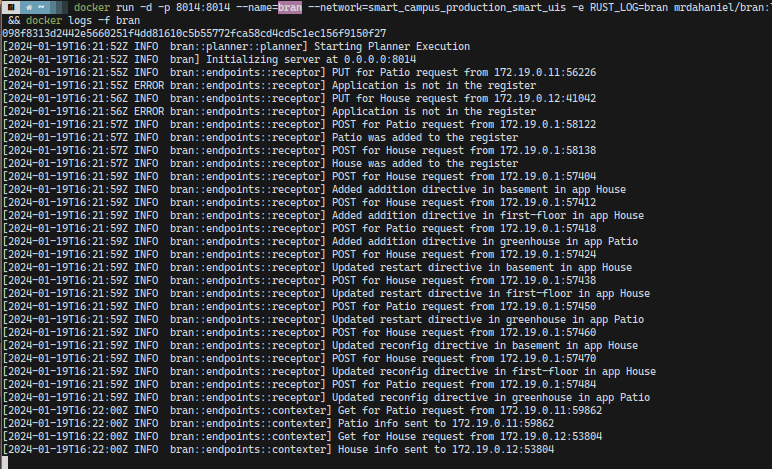
\includegraphics[width=\linewidth]{images/BranBScenarioDeclarition.png}
    \vspace{-4mm}
\end{figure}

Seguidamente, como se observa en la figura \ref{fig:Looker2Apps}, se desplegaron los servicios de \textit{Looker} para cada una de las aplicaciones a monitorear. Ya con esta base lista, y como se definió en los pasos a seguir, se desplegaron de manera manual, un total de 3 servicios \textit{Mocker} con configuraciones específicas (tanto de los datos que estos reportaban, como de los tiempos de reporte) con el fin de cumplir con los requerimientos de datos definidos para las dos aplicaciones. 

\begin{figure}[ht]
    \centering
    \caption{Dos instancias de looker monitoreando las aplicaciones declaradas}
    \label{fig:Looker2Apps}
    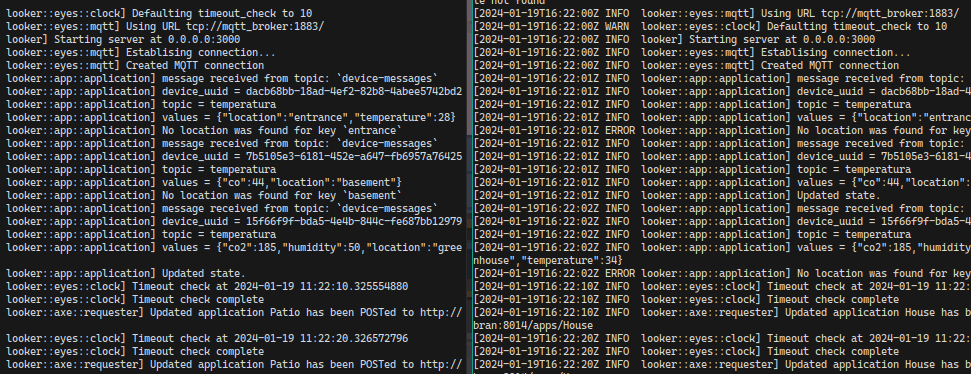
\includegraphics[width=\linewidth]{images/Looker2Apps.png}
    \vspace{-4mm}
\end{figure}

Como era de esperarse, con las configuraciones hechas a la medida de las aplicaciones, el estado de estas era \textit{Coherent}, sin la necesidad de ningún tipo de cambios en los dispositivos. Siendo así, como se ve en la figura \ref{fig:KillThemAll}, se matan los 3 contenedores desplegados, y se elimina uno de ellos.

\begin{figure}[ht]
    \centering
    \caption{Se matan los contenedores con los servicios iniciales}
    \label{fig:KillThemAll}
    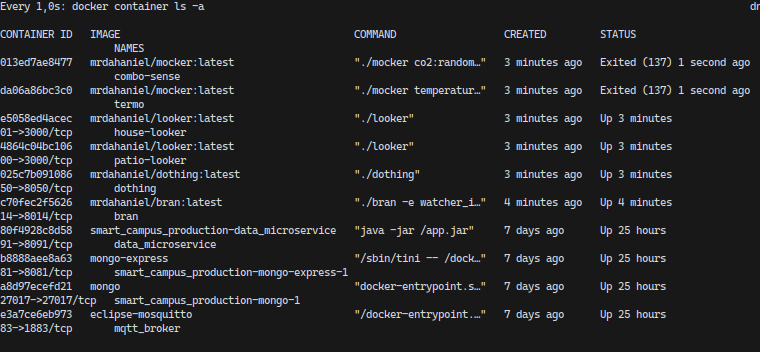
\includegraphics[width=\linewidth]{images/Killing.png}
    \vspace{-4mm}
\end{figure}

La figura \ref{fig:FindAny}, muestra el como \textit{Bran}, define las órdenes para reiniciar los servicios para traer la aplicación a un estado nuevamente. En condiciones normales, se esperaría que esto sea lo único a realizar para adaptar la arquitectura, sin embargo, este no fue el caso.

\begin{figure}[ht]
    \centering
    \caption{Bran intenta reiniciar los contenedores}
    \label{fig:FindAny}
    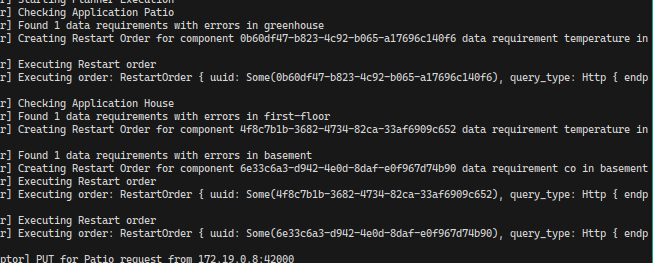
\includegraphics[width=\linewidth]{images/BranOrdersRestarts.png}
    \vspace{-4mm}
\end{figure}

\newpage

Ya que los contenedores no fueron desplegados, o ha sido modificados, de ninguna manera por \textit{DoThing}, no estos no están mapeados. Siendo así, como se ve en la figura \ref{fig:CantFindAny}, es necesario buscar los contenedores en la red, pero, al estar los servicios muertos, y depender de la consulta \textit{Http} para poder identificarlos, no puede encontrarlos.


\begin{figure}[H]
    \centering
    \caption{DoThing no puede encontrar los contenedores}
    \label{fig:CantFindAny}
    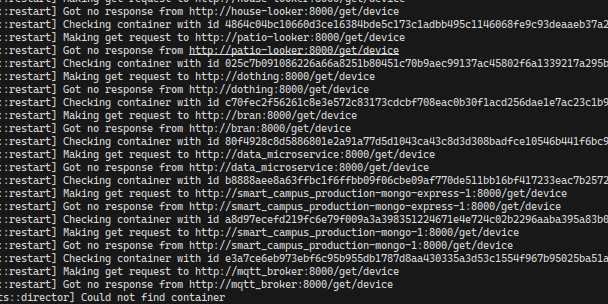
\includegraphics[width=\linewidth]{images/CantFind.png}
    \vspace{-4mm}
\end{figure}

Esto demuestra otra de las falencias con la implementación realizada, que es la búsqueda del crecimiento de la fase de conocimiento. El haber identificado los componentes, antes de que se presentaran problemas, hubiera posibilitado la ejecución de órdenes cuando los servicios estén caídos. Así mismo, se hubiera podido establecer una búsqueda que no dependiera del estado de los componentes, quizás usando tags.

El resultado final, es que \textit{Bran}, al no poder actuar de otra manera, ordena acciones de adición para suplir los componentes. Esto, eventualmente, resulta en el regreso de la aplicación a un estado válido, pero sigue sin ser lo ideal.

\begin{figure}[H]
    \centering
    \caption{Bran crea órdenes de adicción}
    \label{fig:HadToAdd}
    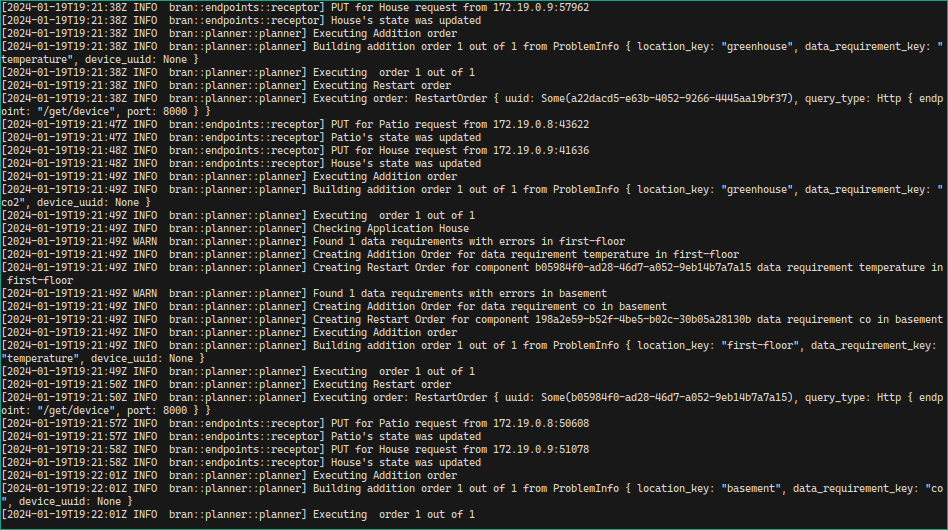
\includegraphics[width=\linewidth]{images/ReLaunchIT.png}
    \vspace{-4mm}
\end{figure}